\documentclass[12pt,fleqn]{article}
\usepackage[portuguese]{babel}
\usepackage{xiiiemc}
\usepackage{natbib}
\usepackage{amsfonts}
\usepackage{amsmath}
\usepackage{mathtools}
\usepackage{fancyhdr}
\usepackage{color}
\usepackage{wallpaper} 
\usepackage{titlesec}   %% Define space between paragraph e section
\usepackage{float} 	%% Use to fix Figure or Table: ex: \begin{table}[H]
\usepackage{listings}
\usepackage{listingsutf8}
\usepackage{siunitx}
\usepackage{subfigure}
\usepackage{enumitem}
\usepackage{graphicx}
\usepackage{verbatim}
\usepackage{tikz}
\usepackage{lipsum}
\usepackage[hyphens]{url}
\usepackage[all]{xy}
\urlstyle{same}
\lstset{
  literate=% %configuration alfabeth  brazilian 
  {\'a}{{\'a}}1
  {\'i}{{\'i}}1
  {\~a}{{\~a}}1
  {\^a}{{\^a}}1
  {\^e}{{\^e}}1,
  basicstyle = \small,
  mathescape % math mode
}

\usepackage{caption}

%%%%Don't edit this block. It reduces the spacing between the lines of the references
\let\OLDthebibliography\thebibliography
\renewcommand\thebibliography[1]{\OLDthebibliography{#1} \setlength{\parskip}{0pt}\setlength{\itemsep}{0pt plus 0.3ex}}
%%-----------------------------------------------EDIT-----------------------------------------------
  \title{UM CASO DE ESTUDO COMPUTACIONAL PARA O DESPACHO EL\'ETRICO DE UM MODELO HIDROT\'ERMICO}%%-----------------------------------------------EDIT----------------------------------------------
\author
    {\rm \begin{tabular}{l} 
    \textbf{Jefferson Bezerra dos Santos}$^{1}$ - {\textnormal jeffersonsantos@ppgmmc.ci.ufpb.br}\\%
    \textbf{Camila Mara Vital Barros}$^{2}$ - {\textnormal camila.barros@ci.ufpb.br}\\
    \textbf{S\'ergio de Carvalho Bezerra}$^{3}$ - {\textnormal sergio@ci.ufpb.br}\\
    {\fontsize{11}{0}\selectfont $^{1}$ {\begin{tabular} {l} Programa de P\'os-gradua\c c\~ao em  Modelagem Matem\'atica e Computacional, Centro de Inform\'atica,\\
    Universidade Federal da Para\'iba - Jo\~ao Pessoa, PB, Brasil.\end{tabular}}}\vspace*{0.07cm} \\
    {\fontsize{10}{0}\selectfont $^{2}$ \begin{tabular}{l} Departamento de Sistemas de Computa\c c\~ao, Centro de Inform\'atica,\\
    Universidade Federal da Para\'iba - Jo\~ao Pessoa, PB, Brasil. \end{tabular}}\vspace*{0.07cm}\\
    {\fontsize{11}{0}\selectfont $^{3}$ \begin{tabular}{l} Departamento de Computa\c c\~ao Cient\'ifica, Centro de Inform\'atica,\\ 
    Universidade Federal da Para\'iba - Jo\~ao Pessoa,
  PB, Brasil.\end{tabular}}
  \end{tabular}}
%%----------------------------------------------------------------------------------------------

\fancypagestyle{firspagetstyle}
{
	\lhead{}
	\fancyhead[C]{%
		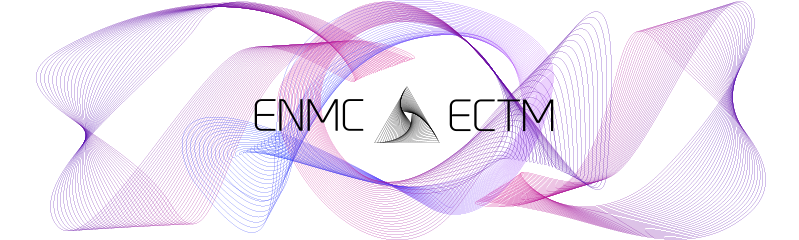
\includegraphics[width=1\linewidth]{logo}\\%
		{\scriptsize \fontfamily{phv}\fontseries{b}\selectfont \color[rgb]{0.45,0.45,0.45}
		08 a 11 de Outubro de 2019\\
		Universidade Federal de Juiz de Fora\\
		Juiz de Fora - MG\\
	    }
	}
	\renewcommand{\headrulewidth}{0.0pt}
	\fancyfoot[C]{\footnotesize \parbox{15cm} {\centering  \fontsize{7.5}{0}\selectfont \it Anais do XXII ENMC – Encontro Nacional de Modelagem Computacional e X ECTM – Encontro de Ciências e Tecnologia de Materiais\\Juiz de Fora, MG – 08 a 11 Outubro 2019}} % \ttfamil
	\rhead{}
}

\begin{document}
% Configuracao para o espacamento entre todas a equacoes
% Modifique o parametro pt para o espaco desejado
%\setlength{\abovedisplayskip}{5pt}
%\setlength{\belowdisplayskip}{5pt}
\setlength{\jot}{1pt}
%\setlength{\abovedisplayshortskip}{0pt}
%\setlength{\belowdisplayshortskip}{0pt}

\maketitle
\thispagestyle{firspagetstyle}

\fancyhead[L]{\footnotesize{\fontsize{7.5}{0}\selectfont \it XXII ENMC e X ECTM\\
	08 a 11 de Outubro de 2019\\
	Universidade Federal de Juiz de Fora – Juiz de Fora - MG\\}}
\renewcommand{\headrulewidth}{0.0pt}
\fancyfoot[C]{\footnotesize \parbox{15cm} {\centering  \fontsize{7.5}{0}\selectfont \it  Anais do XXII ENMC – Encontro Nacional de Modelagem Computacional e X ECTM – Encontro de Ciências e Tecnologia de Materiais\\Juiz de Fora, MG – 08 a 11 Outubro 2019}} % \ttfamil
\rhead{}

\begin{abstract}
  Com o aumento da demanda por energia el\'etrica e o apelo das fontes renov\'aveis, grandes avan\c cos tecnol\'ogicos
  s\~ao indispens\'aveis para um crescimento eficiente e sustent\'avel. No Brasil a hidrel\'etrica \'e a principal fonte de gera\c c\~ao de energia. No entanto, devido ao aumento desproporcional da demanda e a escassez de chuvas, tem sido necess\'ario a ativa\c c\~ao de termel\'etricas para suprir a demanda. Consequentemente, isto acarreta em um aumento na fatura
  dos consumidores residenciais. Neste contexto, este trabalho tem como finalidade analisar, as consequ\^encias que o aumento da demanda e varia\c c\~oes de produtibilidade 
  associados a problemas energ\'eticos, podem ocasionar no gerenciamento do balan\c co energ\'etico. Vislumbrando a necessidade de realizar um gerenciamento adequado do despacho de energia, de modo a minimizar os custos da gera\c
  c\~ao e uma diminui\c c\~ao do impacto ambiental, neste trabalho foi proposto um estudo baseado em Programa\c c\~ao
  Din\^amica Dual Estoc\'astica para sistemas hidrot\'ermicos (hidrel\'etricas e termel\'etricas). De fato, ao variar a produtibilidade e a demanda se identifica qual a configura\c c\~ao de despacho que apresenta o menor custo esperado para a gera\c c\~ao do sistema. 
\end{abstract}

\palavra {\em{Gera\c c\~ao de Energia, Demanda, Modelo Hidrot\'ermico, Planejamento, Progra-ma\c c\~ao Din\^amica Dual Estoc\'astica.}}
\pagestyle{fancy}

\section{INTRODU\c C\~AO}
A crescente necessidade pelo atendimento \`a demanda tem ocasionado um aumento da complexidade dos
sistemas de gera\c c\~ao de energia el\'etrica. Em contrapartida, a pesquisa por uma gera\c c\~ao de energia que favore\c
ca o desenvolvimento sustent\'avel tornou-se um dos principais temas debatidos no cen\'ario internacional. O sistema brasileiro \'e constitu\'ido predominantemente por um sistema interligado
hidrot\'ermico, tendo como caracter\'isticas principais o interc\^ambio de energia entre regi\~oes e a possibilidade de
complementaridade existente entre as hidrel\'etricas e as termel\'etricas (Tolmasquim, 2016). Em um planejamento hidrot\'ermico os aspectos
de relev\^ancia s\~ao: acoplamento espacial, acoplamento temporal e o componente estoc\'astico dos reservat\'orios. Em cada
est\'agio do planejamento \'e necess\'aria a tomada de decis\~ao fazendo-se a escolha pela quantidade gerada de energia
proveniente das termel\'etricas e das hidrel\'etricas. Neste
contexto, atualmente destaca-se a Programa\c c\~ao Din\^amica Dual
Estoc\'astica (PDDE), pois possibilita uma flexibilidade para a descri\c c\~ao do acoplamento temporal e espacial existente entre as
usinas hidrel\'etricas, al\'em de permitir o  planejamento em v\'arios cen\'arios de aflu\^encias proporcionando-se a
modelagem da incerteza dos reservat\'orios. Contudo, dependendo da quantidade elevada de cen\'arios  para o planejamento
nem sempre \'e poss\'ivel que a t\'ecnica de PDDE obtenha uma configura\c c\~ao \'otima para todos os cen\'arios
considerados, tornando-se sua principal desvantagem.

Diversos trabalhos na literatura utilizam a PDDE como forma de planejamento. Um estudo recente da t\'ecnica
de constru\c c\~ao de \'arvore de cen\'arios para a PDDE pode ser encontrado em (Rebennack, 2016). O estudo sobre modelagem hidrot\'ermica n\~ao convexa utilizando PDDE para restri\c c\~oes n\~ao lineares envolvendo reservat\'orios de
hidrel\'etricas \'e encontrado em (Cerisola \& Latorre \& Ramos,
2012). E uma an\'alise comparativa entre Programa\c c\~ao Din\^amica Primal Estoc\'astica e PDDE para modelo
hidrot\'ermico de longo prazo \'e descrita em (Martinez \&
Soares, 2004). 

Neste trabalho propõe-se a analisar os pontos cr\'iticos de demanda e de produtibilidade em modelos hidrot\'ermicos que utilizam a PDDE.
Tendo como intuito verificar quais as consequ\^encias nas varia\c c\~oes da demanda e da produtibilidade no valor total do custo esperado. Vale destacar a obten\c c\~ao de duas configura\c c\~oes de despacho considerando-se o aspecto macro, ou seja, ordem de acionamento das hidrel\'etricas e das termel\'etricas, com o aumento da demanda e dos n\'iveis de produtibilidade.  Ao final se detecta qual cen\'ario apresenta o menor custo esperado de produ\c c\~ao de gera\c c\~ao de energia el\'etrica, dentro das situa\c c\~oes modeladas.

 Este trabalho \'e
subdividido da seguinte maneira: Na Se\c c\~ao 2 foi abordada a configura\c c\~ao do despacho do Brasil; Na se\c c\~ao 3
\'e abordada a Programa\c c\~ao Din\^amica Dual Estoc\'astica; Na se\c c\~ao 4 \'e abordada a an\'alise das simula\c
c\~oes; Na se\c c\~ao 5 as conclus\~oes e trabalhos futuros. 

\section{DESPACHO DE ENERGIA}
A an\'alise dos fatores que envolvem a matriz energ\'etica brasileira sobre os aspectos relacionados \`a demanda e a oferta possui um grau de complexidade elevado. Um dos principais elementos que ocasionam empecilhos \'e a depend\^encia h\'idrica que ocorre no setor energ\'etico brasileiro (Tolmasquim, 2016). O Brasil possui o Sistema Interligado Nacional (SIN) que corresponde as
regi\~oes Sul, Sudeste, Centro-Oeste, Nordeste e parte do Norte. Sendo este, respons\'avel por gerar cerca de $96,6\%$ de toda a capacidade de produ\c c\~ao de energia do Brasil (Atlas de
energia el\'etrica no Brasil, 2008). Uma das vantagens da ado\c c\~ao do SIN deve-se a possibilidade de interc\^ambio
energ\'etico, isto \'e, regi\~oes que sofrem com problemas no abastecimento  de energia devido a algum motivo externo
podem ser auxiliadas por outras regi\~oes. Uma outra possibilidade \'e a opera\c c\~ao de usinas hidrel\'etricas e termel\'etricas no
regime de complementaridade, ou seja, as termel\'etricas s\~ao ativadas para suprir demanda quando por algum motivo as
hidrel\'etricas n\~ao conseguem atingir a meta, evitando-se preju\'izos na oferta. O sistema de energia brasileiro tamb\'em \'e constitu\'ido pelos sistemas isolados localizados principalmente na regi\~ao Norte,
estados como Amazonas, Roraima, Acre, Amap\'a e Rond\^onia. Esta denomina\c c\~ao deve-se por n\~ao estarem interligados ao
SIN e por n\~ao permitirem um interc\^ambio com outras regi\~oes devido as caracter\'isticas geogr\'aficas. O
funcionamento dos
sistemas isolados \'e predominantemente t\'ermico. Os custos para a gera\c c\~ao de energia nesses sistemas s\~ao
superiores ao SIN (Atlas de
energia el\'etrica no Brasil, 2008).

 A produ\c c\~ao de eletricidade no sistema brasileiro tem como objetivo principal minimizar
os custo de opera\c c\~ao e garantir o suprimento de energia em todo o pa\'is (Tolmasquim, 2016). Devido SIN ser
constitu\'ido predominantemente por um sistema hidrot\'ermico este \'e afetado pela incerteza associada a pluviosidade
das regi\~oes que o constituem (Atlas de
energia el\'etrica no Brasil, 2008). No entanto, a demanda do sistema deve ser garantida de forma a n\~ao prejudicar o
abastecimento, ao mesmo tempo a gera\c c\~ao term\'eletrica associada aos sistemas isolados possui um custo elevado. Este custo deve ser considerado para n\~ao ocasionar um
aumento desagrad\'avel no pre\c co  associado ao sistema de energia brasileiro. 
Neste contexto, o planejamento eficiente do sistema energ\'etico observando caracter\'isticas como, demanda, oferta e
  as configura\c c\~oes do sistema \'e conhecido na literatura como o despacho de energia. Para sistemas
 hidrot\'ermicos as caracter\'isticas do despacho podem ser resumidas no dilema do
 ``operador'' dado pelo diagrama a seguir.
 {\setlength{\jot}{2pt}
 \begin{figure}[!h]
 \centering
 \resizebox{0.4\textwidth}{!}{%
  \xymatrix@=1.0em{
	& & *+[F]{\text{CHUVA}} \ar[r]& *+[F]{\text{DECIS\~AO CORRETA}}\\
	& *+[F]{\text {USAR \ RESERVAT\'ORIO}} \ar[ur] \ar[dr] & &\\
	& & *+[F]{\text{SECA}} \ar[r] & *+[F]{\text{PREJU\'IZO}} \\
	*+ [F]{\text {OPERADOR}} \ar[uur] \ar[ddr] & & & \\
	& & *+[F]{ \text {CHUVA}} \ar[r] & *+ [F]{\text{PREJU\'IZO}}\\
	& *+ [F]{\text {USAR TERMEL\'ETRICA}} \ar[ur] \ar[dr]& &\\
	& & *+[F] {\text {SECA}} \ar[r] & *+[F]{\text{DECIS\~AO CORRETA}}
 }}
 \caption {Dilema do operador.}  
 \label{fig1}
 \end{figure}
}
Conforme o diagrama o operador do sistema pode ter preju\'izo associado a sua escolha dado o componente estocastico
relacionado aos
reservat\'orios das hidrel\'etricas. Pela complexidade do sistema hidrot\'ermico
brasileiro este tipo de decis\~ao possui um grau de dificuldade que transcede a simplicidade. Nesta perspectiva um dos modelos de
planejamento desenvolvido para lidar com a tomada de decis\~ao de curto prazo foi desenvolvido pelo Centro de
Pesquisas de Energia El\'etrica (Cepel), o chamado Modelo de Planejamento de Sistemas Interligados de
Curto Prazo (DECOMP). Esse modelo fundamenta-se na t\'ecnica conhecida na literatura como Programa\c c\~ao Din\^amica
Dual Estoc\'astica.

\section{Programa\c c\~ao Din\^amica Dual Estoc\'astica}
\subsection{Otimiza\c c\~ao}
No planejamento de um sistema energ\'etico hidrot\'ermico o sistema deve preservar as metas de gera\c c\~ao para suprir a demanda e minimizar o valor esperado do custo de
opera\c c\~ao ao longo do per\'iodo de estudo. As caracter\'isticas mencionadas configuram o despacho de energia
. Diante das possibilidades de configura\c c\~oes poss\'iveis para o sistema (sequ\^encia de acionamento das hidrel\'etricas e das termoel\'etricas com o aumento da demanda para uma produtibilidade fixa) deseja-se obter a combina\c
c\~ao na qual o valor do custo
associdado seja m\'inimo. Portanto, o despacho de energia trata-se de um problema de otimiza\c c\~ao. No estudo da
teoria da otimiza\c c\~ao existe uma fun\c c\~ao $f$ ao qual intenta-se obter
quando poss\'ivel seu minimizador (Izmailov \& Solodov, 2014). Um entendimento intuitivo pode ser dado pelas figuras a seguir:

\begin{figure}[!h]
  \centering
	\resizebox{0.3\textwidth}{!}{%
\begin{tikzpicture}
  \draw [->, thick, black] (0,0)--(8,0) node[right] {$x$};
  \draw [->, thick, black] (0,0)--(0,4) node[above] {$f$};
  \draw [thick, black] (0,1)--(1,3);
  \draw [thick, black] (1,3)--(2,0.5) node[above1,xshift = 3,yshift = 16] {$G$};
  \draw [thick, black](2,0.5)--(4,3);
  \draw [thick, black](4,3)--(5,2) node[below left] {$L$};
  \draw [thick, black](5,2)--(6,3)--(8,3)node[above,yshift=8] {$D$};
  \draw [ultra thick, black](2,0.5) circle (0.5mm);
  \draw [ultra thick, black](5,2) circle (0.5mm);
  \draw [ultra thick, black](5,2) circle (0.5mm);
  \draw [dashed, black](2,0.5)--(0,0.5) node[left] {$f(x_g)$} ;
  \draw [dashed, black](2,0.5)--(2,0) node[below] {$x_g$};
  \draw [dashed, black] (1.5,1.8)--(1.5,0) node[below] {$x_1$};
  \draw [dashed, black] (1.5,1.8)--(0.0,1.8) node[left] {$f(x_1)$};
  \draw [dashed, black](3.8,2.7)--(3.8,0) node[below] {$x_2$};
  \draw [dashed, black](3.5,2.7)--(0.0,2.7) node[above left] {$f(x_2)$};
  \draw [dashed, black](5,2)--(0,2) node[above left] {$f(x_l)$};
  \draw [dashed, black](5,2)--(5,0) node[below] {$x_l$};
  \draw [thick, black](4,0) circle (0.01mm) node[below,yshift=-20] {Caso 1};
\end{tikzpicture}
}
\resizebox{0.3\textwidth}{!}{%
\begin{tikzpicture}
  \draw [->, thick, black] (0,0)--(8,0) node[right] {$x$};
  \draw [->, thick, black] (0,0)--(0,4) node[above] {$f$};
  \draw [thick, black] (0,1)--(1,3);
  \draw [thick, black] (1,3)--(2,0.5) node[above1,xshift = 3,yshift = 16] {$G$};
  \draw [thick, black](2,0.5)--(4,3);
  \draw [thick, black](2,0.5)--(4,3);
  \draw [thick, black](4,3)--(5,2) node[below left] {$L$};
  \draw [thick, black](5,2)--(6,3)--(8,3)node[left,yshift=8] {$D$};
  \draw [ultra thick, black](2,0.5) circle (0.5mm);
  \draw [ultra thick, black](4.5,0) circle (0.1mm) node[below]{$x_d$};
  \draw [dashed, black](5,2)--(5,0) node[below] {$x_l$};
  \draw [ultra thick, black](5,2) circle (0.5mm);
  \fill [black, draw=black, opacity = 0.4] (4.5,0) rectangle (8,4);
 %% \draw [thick, black](5,0) circle (0.2mm) node[below] {$x_l$};
  \draw [dashed, black](2,0.5)--(0,0.5) node[left] {$f(x_g)$};
  \draw [dashed, black](2,0.5)--(2,0) node[below] {$x_g$};
  \draw [dashed, black] (1.5,1.8)--(1.5,0) node[below] {$x_1$};
  \draw [dashed, black] (1.5,1.8)--(0.0,1.8) node[left] {$f(x_1)$};
  \draw [dashed, black](3.8,2.7)--(3.8,0) node[below] {$x_2$};
  \draw [dashed, black](3.5,2.7)--(0.0,2.7) node[above left] {$f(x_2)$};
  \draw [dashed, black](5,2)--(0,2) node[above left] {$f(x_l)$};
  \draw [thick, black](4,0) circle (0.01mm) node[below,yshift=-20] {Caso 2};
  \end{tikzpicture}
}
\caption{Minizador $G$, minizador $L$ e Conjunto $D$.}
\label{fig2}
\end{figure}
Analisando a Figura (\ref{fig2}) nota-se dois casos espec\'ificos: em cada caso o que muda \'e o dom\'inio da regra de associa\c c\~ao, esse dom\'inio \'e o conjunto vi\'avel. Para o primeiro caso \'e verdadeira a afirma\c c\~ao $f(x_g)
\leq f(x)$ para qualquer $x$ do dom\'inio maximal. No segundo caso, se restringe o dom\'inio, ou seja, muda-se o conjunto vi\'avel (para valores de $x$ pertencentes ao conjunto cinza da Figura (\ref{fig2})). No segundo caso da Figura (\ref{fig2}) perceba a mudan\c ca do conjunto vi\'avel o que implica ser o ponto $L$ o novo minimizador, para o novo conjunto vi\'avel. Pois, $f(x_l) \leq f(x)$ para todo $x$ no segundo conjunto vi\'avel. O  minimizador do problema de
otimiza\c c\~ao dado o conjunto vi\'avel $D$ \'e conhecido como ponto de \'otimo. Sua nomenclatura comum \'e dada por ${x}^{*}$.  De forma equivalente pode-se
representar o problema por,
\begin{align}
\label {min1}
  \min_{x\in D} f(x),
\end{align}
onde ${x}^{*}$ satisfaz:
\begin{align}
	  f({x}^{*}) \leq f(x) \mbox{ para }x \in D. \nonumber
\end{align}

Para o presente estudo \'e suficiente considerar o conjunto $D$ como sendo um conjunto poliedral. De uma forma bem grosseira, a ideia \'e evitar
poss\'iveis ``fissuras'' em nosso conjunto de restri\c c\~oes. Um conjunto  \'e dito poliedral  quando se pode represent\'a-lo como um conjunto de solu\c c\~oes de um sistema finito de equa\c c\~oes e inequa\c c\~oes lineares (Izmailov \& Solodov, 2014). Por exemplo,
\begin{align}
  D = \left\{ x \in \mathbb{R}^{n}; Ax = a, Bx \leq b\right\},\nonumber
\end{align}
onde $A \in R(l,m)$, $B \in R(m,n)$, $a \in \mathbb{R}^{n}$, e $b \in \mathbb{R}^{m}$ adotando-se que $R(l,m)$ representa o
espa\c co de matrizes com $l$ linhas, e $m$ colunas. Dada que $f$ na Eq.(\ref {min1}) \'e uma fun\c c\~ao linear e $D$ um conjunto
poliedral. Ent\~ao, na Teoria da Otimiza\c c\~ao, tais problemas s\~ao denotados ser Problemas de Programa\c c\~ao Linear. O problema de despacho de energia, para o caso determin\'istico pertence a essa categoria. Por fim, para problemas de otimiza\c c\~ao de uma forma geral o conceito de dualidade \'e
indispens\'avel. Considerando-se um problema de Programa\c c\~ao Linear que ser\'a chamado de problema primal,
\begin{align}
  \displaystyle\min_{ x \in D = \left\{ x \in \mathbb{R}^{n}; Bx \geq b \right\}} \left < c,x \right >, 
  \label{min2}
\end{align}
onde $B \in R(m,n), c \in \mathbb{R}^{n}$ e $b \in \mathbb{R}^{n}$ onde ``$< >$'', representar o produto interno Euclidiano.
O problema dual para Eq. (\ref{min2}) \'e definido por,
\begin{align*}
  \max_{\mu \in \Delta = \left\{ \mu \in \mathbb{R}_+^m;
  {B}^{T} \mu = c \right\}} \left < b, \mu \right > .
\end{align*}

A grande import\^ancia da dualidade para a Programa\c c\~ao Linear deve-se ao fato que em certas circunst\^ancias o valor \'otimo do problema dual \'e equivalente ao do
problema primal e na maioria dos casos o problema dual possui uma estrutura menos complexa (Izmailov \& Solodov, 2014). Uma
vez que o instrument\'ario necess\'ario foi desenvolvido pela teoria de otimiza\c c\~ao. Assim, pode-se estudar o problema do despacho de
energia usando o modelo desenvolvido pelo Centro de Pesquisas de Energia El\'etrica (Cepel), denominado modelo DECOMP. 

\subsection{Modelo de Planejamento de Opera\c c\~ao de Sistemas Hidrot\'ermicos Interligados de Curto Prazo}
O despacho de energia em sistemas hidrot\'ermicos envolve um conjunto de fatores que dificultam a tomada de decis\~ao, 
n\~ao somente os n\'iveis dos reservat\'orios devem ser considerados, mas tamb\'em o acoplamento espacial existente entre as usinas
hidrel\'etricas. Consequentemente, usinas a jusante possuem depend\^encia de usinas a montante e o acoplamento temporal, isto
\'e,
decis\~oes no momento de planejamento podem ocasionar consequ\^encias no futuro, tais fatores  precisam ser observados para
o despacho hidrot\'ermico. A figura a seguir representa a rela\c c\~ao existente entre as usinas. 
\begin{figure}[!htpb]
  \centering
  \resizebox{0.4\textwidth}{!}{%
  \begin{tikzpicture}
  % Desenho da cascata
  \draw [ultra thick,black] (7.2,9.0) circle (0.01mm) node[above]{Usinas em cascata};
  %
  % Desenho da montante
  \draw (-1.0,7.0) rectangle (0.6, 7.5) 
  node[below left] {\footnotesize Montante};
  %
  % Desenho da jusante

  \draw [thick, black]  (-1,0)--(-1,7);
  \draw [thick, black]  (-1,0)--(7,0);
  \draw [fill=darkgray] (-1.0,7.0) .. controls (0.5,7.0) .. (0.5,6.5);
  \draw [fill=darkgray] (0.0,7.0) .. controls (0.5,7.0) .. (0.5,6.5);
  \draw [fill=darkgray] (0.5,6.5) .. controls (1.0,6.5) .. (1.0,6.0);
  \draw [fill=darkgray] (1.0,6.0) .. controls (1.5,6.0) .. (1.5,5.5);
  \draw [fill=darkgray] (1.5,5.5) .. controls (2.0,5.5) .. (2.0,5.0);
  \draw [fill=darkgray] (2.0,5.0) .. controls (2.5,5.0) .. (2.5,4.5);
  \draw [fill=darkgray] (2.5,4.5) .. controls (3.0,4.5) .. (3.0,4.0);
  \draw [fill=darkgray] (3.0,4.0) .. controls (3.5,4.0) .. (3.5,3.5);
  \draw [fill=darkgray] (3.5,3.5) .. controls (4.0,3.5) .. (4.0,3.0);
  \draw [fill=darkgray] (4.0,3.0) .. controls (4.5,3.0) .. (4.5,2.5);
  \draw [fill=darkgray] (4.5,2.5) .. controls (5.0,2.5) .. (5.0,2.0);
  \draw [fill=darkgray] (5.0,2.0) .. controls (5.5,2.0) .. (5.5,1.5);
  \draw [fill=darkgray] (5.5,1.5) .. controls (6.0,1.5) .. (6.0,1.0);
  \draw [fill=darkgray] (6.0,1.0) .. controls (6.5,1.0) .. (6.5,0.5);
  \draw [fill=darkgray] (6.5,0.5) .. controls (7.0,0.5) .. (7.0,0.0);
  \draw [fill=darkgray,line width=0.1pt, opacity=100] (0,7)--(7,0);
  \filldraw [darkgray, line width=2.0pt] (0,7)--(7,0)--(-1,0)--(-1,7);
  %
  % Desenho de H1 
  \draw [thick, black] (1.7,6.5) circle (0.01mm) node [above]{\footnotesize $H1$};
  \draw [thick, black] (0.5,6.5)--(2.5,6.5);
  \draw [thick, black] (1.7,6.5) circle (0.01mm) node [below]{\footnotesize $R1$};
  \draw [thick, black] (2.5,6.5)--(2.0,5.4);
  
  \draw [fill=blue](1.40,6.0)--(2.25,6.0)--(2.0,5.4)--(1.47,5.4);
  % 
  % Desenho de H2
  \draw [thick, black] (6.0, 2.0) circle (0.01mm) node[above]{ \footnotesize $H2$};
  \draw [fill=darkgray] (5.0,2.0) -- (7.0,2.0);
  \draw [thick, black] (6.0,2.0) circle (0.01mm) node [below]{\footnotesize $R2$};
  \draw [fill=darkgray] (7.0,2.0) -- (6.39,1.0);
  \draw [fill=blue] (5.9,1.5) -- (6.7,1.5) --(6.39,1.0) -- (5.9, 1.0); 
  %
  % Desenho fio de agua
  \filldraw [blue, line width=1pt] (0.4, 7.0) .. controls (0.6, 7.0) .. (0.5,6.5);

  \draw [blue, ultra thick] (0.0,7.0) .. controls (0.5,7.0) .. (0.5,6.5);
  \draw [blue, ultra thick] (0.5,6.5) .. controls (1.0,6.5) .. (1.0,6.0);
  \draw [blue, ultra thick] (1.0,6.0) .. controls (1.5,6.0) .. (1.5,5.5);
  \draw [blue, ultra thick] (1.5,5.5) .. controls (2.0,5.5) .. (2.0,5.0);
  \draw [blue, ultra thick] (2.0,5.0) .. controls (2.5,5.0) .. (2.5,4.5);
  \draw [blue, ultra thick] (2.5,4.5) .. controls (3.0,4.5) .. (3.0,4.0);
  \draw [blue, ultra thick] (3.0,4.0) .. controls (3.5,4.0) .. (3.5,3.5);
  \draw [blue, ultra thick] (3.5,3.5) .. controls (4.0,3.5) .. (4.0,3.0);
  \draw [blue, ultra thick] (4.0,3.0) .. controls (4.5,3.0) .. (4.5,2.5);
  \draw [blue, ultra thick] (4.5,2.5) .. controls (5.0,2.5) .. (5.0,2.0);
  \draw [blue, ultra thick] (5.0,2.0) .. controls (5.5,2.0) .. (5.5,1.5);
  \draw [blue, ultra thick] (5.5,1.5) .. controls (6.0,1.5) .. (6.0,1.0);
  \draw [blue, ultra thick] (6.0,1.0) .. controls (6.5,1.0) .. (6.5,0.5);
  \draw [blue, ultra thick] (6.5,0.5) .. controls (7.0,0.5) .. (7.0,0.0);
  %
  % Desenho da legenda
   \node [draw,align=justify, minimum size=2cm]() at (12.5,6.0) {\footnotesize $H1$-\footnotesize Hidrel\'etrica 1 \\
  \footnotesize $R1$-\footnotesize Reservat\'orio de H1 \\ 
  \footnotesize $H2$-\footnotesize Hidrel\'etrica 2 \\
  \footnotesize $R2$-\footnotesize Reservat\'orio de H2};
  %\draw (9.5,4.5) rectangle (13.5,7.0); 
  %\draw (11.0,6.5) circle (0.01mm) node[] {\footnotesize $H1$-\footnotesize Hidrel\'etrica 1};
  %\draw (11.3,6.0) circle (0.01mm) node[] {\footnotesize $R1$-\footnotesize Reservat\'orio de H1};
  %\draw (11.0,5.5) circle (0.01mm) node[] {\footnotesize $H2$-\footnotesize Hidrel\'etrica 2};
  %\draw (11.3,5.0) circle (0.01mm) node[] {\footnotesize $R2$-\footnotesize Reservat\'orio de H2};
  %
  % Desenho do acoplamento temporal
  \draw (1.4,6)--(6,1.4);
  \draw [thick, black] (3.6,3.6) circle (0.01mm) node[above, rotate=315]{\fontsize{9}{12}\selectfont {Depend\^encia entre os
  reservat\'orios}};
  \draw [->,thick, black,rotate around={-50:(4.0,4.0)}]
	(4.0,4.0)--(4.0,4.7)node[above, rotate=315]{\footnotesize acoplamento espacial};
	\draw [->,thick, black](2.25,6.0)--(2.25,7.5) node[above,align=center]{\footnotesize N\'ivel do reservat\'orio 
	\\ \quad \footnotesize depende decis\~ao do operador};
	\draw [->,thick, black] (4.2,8.2) -- (5.0,8.2) node[right] {\footnotesize acoplamento temporal};
	%
	% Desenho da Jusante
	\draw (7.0,0.0) rectangle (8.5, 0.5);
	\draw (7.8,0.3) circle (0.01mm) node[]{\footnotesize{} Jusante};  
\end{tikzpicture}
}
  \caption{Representa\c c\~ao do acoplamento espacial e temporal.}
\end{figure}

Na constru\c c\~ao do modelo considera-se primeiramente o caso determin\'istico supondo um problema de opera\c
c\~ao em dois est\'agios de tal forma que 
aflu\^encia em cada usina hidrel\'etrica em qualquer est\'agio do tempo \'e conhecida (DECOMP, 2001). De tal forma,
podendo-se modelar o problema por:
\begin{align}
&\min \langle c_1,x_1\rangle + \langle c_2,x_2\rangle \nonumber \\
&\mbox{tal que: }	A_1 x_1 \geq b_1 \\
&E_1 x_1 + A_2 x_2 \geq b_2 \nonumber
\label{p1}
\end{align}
\begin{itemize}[itemsep=-2pt]
  \item $c_1$ e $c_2$ s\~ao vetores que representam os custos relacionado aos est\'agios 1 e 2 respectivamente;
  \item $x_1$ e $x_2$ s\~ao vetores que representam as decis\~oes tomadas nos est\'agios 1 e 2 respectivamente;
  \item $b_1$ e $b_2$  s\~ao os vetores de recursos nos est\'agios 1 e 2 respectivamente;   \item $A_1$ e $A_2$ s\~ao matrizes que representam o acoplamento espacial;
  \item $E_1$ \'e uma matriz que descreve o acoplamento temporal.
\end{itemize}
Este tipo de problema pode ser interpretado como uma decis\~ao em dois est\'agios para sua resolu\c c\~ao \'e
escolhida uma decis\~ao vi\'avel $x_1$ denotada por ${x_1}^{*}$ de tal forma que $A_1{x_1}^{*} \geq b_1$. 
Assim, o problema para decis\~ao do est\'agio 2 pode ser reescrito como, 
\begin{align}
    \label{p2}
  \begin{split}	
 & 	\min \langle c_2,x_2\rangle  \\
&\mbox{tal que: }A_2 x_2 \geq b_2 -{E_1 x_1}^{*}  
  \end{split}
\end{align}
onde a Eq.(\ref {p2}) \'e um problema de Programa\c c\~ao Linear e ${x_1}^{*}$ \'e conhecido. Uma vez representadas as decis\~oes vi\'aveis tomadas no est\'agio 1 do
problema o intuito \'e minimizar o custo da fun\c c\~ao objetivo para o est\'agio 2. Dado que ${x_1}^{*}$ \'e vi\'avel procura-se uma solu\c c\~ao \'otima para $x_2$ representado por
${x_2}^{*}$. A solu\c c\~ao do est\'agio 2 depende das decis\~oes tomadas no est\'agio 1. Portanto, o
problema do est\'agio 2 pode ser visto como uma fun\c c\~ao do 1 est\'agio, isto \'e,
\begin{align}
  \begin{split}	
	\alpha_{1} (x_1) =& \min \langle c_2,x_2\rangle \\
	&\mbox{tal que: }A_2 x_2 \geq b_2 - {E_1 x_1}^{*} 
  \end{split}
    \label{p3}
\end{align}
onde ${\alpha}_{1}$ representa o valor \'otimo para o est\'agio 2. A Eq.(\ref{p1}) pode ser reescrita como se segue,
\begin{align}
  \begin{split}	
  &\min \langle c_1,x_1\rangle + {\alpha}_{1}(x_1) \\
&\mbox{tal que: }	A_1x_1 \geq b_1.
\end{split}
  \end{align}
Aplicando a dualidade na Eq.(\ref{p2}) \'e imediato que,
\begin{align}
  \begin{split}	
 \alpha_{1}(x_1) = &\max \pi (b_2 - E_1x_1 ) \\
	&\mbox{tal que: }\pi A_2  \leq c_2.
  \end{split}
 	\label{p4}
\end{align}

Nas circunst\^ancias do problema a solu\c c\~ao da Eq.(\ref{p4}) \'e equivalente a Eq.(\ref{p2})
nota-se que o conjunto vi\'avel $\pi A_2 \leq c_2$ da Eq.(\ref{p4}) n\~ao depende do valor de $x_1$. Desta forma, os
pontos extremos ou v\'ertices do conjunto vi\'avel podem ser caracterizados por $\pi = \left\{ \pi^1, \pi^2, \dots,
\pi^P \right\}$. Uma vez
que a solu\c c\~ao de um problema de Programa\c c\~ao Linear corresponde  a um v\'ertice do conjunto vi\'avel,
portanto a Eq.(\ref{p4}) pode ser reescrita como se segue,
\begin{align*}
  \begin{aligned}
	{\alpha}_{1}(x_1) = \text {max} \ \ {\pi}^{i} (b_2 - E_1x_1) \\
	{\pi}^{1} \in \left\{ {\pi}^{1}, {\pi}^{2},\dots, {\pi}^{P} \right\}
  \end{aligned}
	\label{p5}
\end{align*}
por fim, a Eq.(\ref{p4}) pode ser reescrita para, 
\begin{align*}
  	\alpha_{1}(x_1) =& \min\alpha \nonumber\\ 
	&\mbox{tais que: }\alpha \geq \pi^{i}(b_2 - E_1 x_1),\nonumber\\ &\mbox{com } i = 1,2, \dots , P
	\label{p6}
\end{align*}
onde $\alpha$ \'e uma vari\'avel escalar. Por fim a Eq.(\ref{p1}) torna-se
\begin{align*}
&\min \langle c_1,x_1\rangle + \alpha \nonumber\\
&\mbox{tal que: }	A_1 x_1 \geq b_1 \nonumber\\
&	\pi^{i}(b_2 - E_1x_1) - \alpha \leq 0\nonumber \\ 
&\mbox{para }	i = 1, 2, \dots , P.
	\label{p7}
\end{align*}

A t\'ecnica para problemas determin\'isticos utilizada \'e conhecida na literatura como a decompo-si\c c\~ao de Benders
(Benders, 1962). A PDDE consiste em uma aplica\c c\~ao da decomposi\c c\~ao de Benders em um problema cuja a
natureza \'e
estoc\'astica. Considerando-se o problema de dois est\'agios similar ao caso anterior, contudo o  est\'agio 2 depende dos valores
que uma ou mais vari\'aveis aleat\'orias podem assumir. Por exemplo, assuma que o vetor $b$ pode assumir dois valores $b_1$ e $b_2$ com
probabilidades $p_1$ e $p_2$ respectivamente, sendo ($p_1 + p_2 = 1$) (DECOMP, 2001). O objetivo \'e encontrar a estrat\'egia que minimiza o
valor do custo esperado. Portanto, o problema fica modelado por:
{\setlength{\belowdisplayskip}{0pt}
\begin{align*}
  z = \min  \langle c_1,x_1\rangle &+ p_1\langle c_2,x_{21}\rangle + p_2\langle c_2,x_{22}\rangle \nonumber\\	
 \mbox{tal que: }&	A_1 x_1 \geq b_1\nonumber \\
	&E_1 x_1 + A_2 x_{21} \geq b_{21} \nonumber\\
	&E_1 x_1 + A_2x_{22} \geq b_{22}
  	\label{pd1}
\end{align*}}%
 Este problema poder ser reescrito como,
{\setlength{\belowdisplayskip}{-4pt}
\begin{align*}
  z = \min  \langle c_1,x_1\rangle + p_1{\omega}_{21} + p_2 {\omega}_{22} \nonumber \\	
	A_1 x_1 \geq b_1
  \end{align*}}%
{\setlength{\abovedisplayskip}{-6pt}
 \setlength{\belowdisplayskip}{0pt}
\begin{align}
  \begin{split}	
  &\omega_{21}(x_1) =\min \langle c_2x_{21}\rangle \\
	& A_2 x_{21} \geq b_{21} - E_1 x_1 
  \end{split}
      \label{pd3}
	\end{align}}%
{\setlength{\abovedisplayskip}{0pt}
\begin{align}
  \begin{split}	
 	&\omega_{22}(x_1) = \min  \langle c_2,x_{22}\rangle \\
	&A_2x_{22} \geq b_{22} - E_1 x_1. 
  \end{split}
     \label{pd4}
   \end{align}}%
Em seguida, aplicando a decomposi\c c\~ao de (Benders, 1962) em Eq.(\ref {pd3}) e Eq.(\ref {pd4}) obtem-se:  
{\setlength{\belowdisplayskip}{-4pt}
\begin{align*}
&\omega_{21}(x_1) = \min  \beta_{1}\nonumber \\
	&\mbox{tal que: }\beta_{1}  \geq {\pi}_{1}^{i}b_{21} - E_1 x_1 \nonumber\\
	&\mbox{para }i = 1,2,\dots, P 
  \end{align*}}%
{\setlength{\abovedisplayskip}{-10pt}
\begin{align*}
 &\omega_{22}(x_1) = \min \beta_{2}\nonumber \\
&\beta_{1}  \geq {\pi}_{2}^{i}b_{22} - E_1 x_1 \nonumber\\
&\mbox{para }i = 1,2,\dots, P 
\end{align*}}%
de maneira an\'aloga ao caso anterior pode-se escrever o problema original estoc\'astico como,
 \begin{align*}
 \begin{aligned}
	\underset {s \backslash a} {\text{min}} \ \ \langle c_1,x_1\rangle + p_1 {\beta}_{1} + p_2 {\beta}_{2} \\
	A_1 x_1 \geq b_1 \\
	{\pi}_{1}^{i}(b_{21} - E_1x_1) - {\beta}_{1} \leq 0 \\ 
	{\pi}_{2}^{j}(b_{22} - E_1x_1) - {\beta}_{2} \leq 0 \\ 
	i = 1, 2, \dots , P \\
	j = 1, 2, \dots , P. \\
  \end{aligned}
  \label{pd5}
\end{align*}
Em poucas linhas, a PDDE faz uma decomposi\c c\~ao no problema original utilizando-se os princ\'ipios de dualidade e a decomposi\c c\~ao
de Benders (Benders, 1962). Isto permite a resolu\c c\~ao do problema original, a partir da solu\c c\~ao de outro
problema. Contudo, este
\'ultimo possui um melhor tratamento computacional, sendo poss\'ivel analisar a influ\^encia da demanda em sistemas
hidrot\'ermicos para v\'arios cen\'arios. A fun\c c\~ao a minimizar  \'e o custo esperado. As restri\c c\~oes do
problema variam em fun\c c\~ao da produtibilidade e da demanda. Em nosso modelo  constatou-se a exist\^encia de duas poss\'iveis sequ\^encias de acionamento das hidrel\'etricas e termel\'etricas, ao aumentarmos a demanda, para uma produtibilidade fixa. Por fim, avalia-se qual situa\c c\~ao apresenta o menor custo esperado. Os dados e os arquivos necessários para o modelo podem ser encontrados na p\'agina do projeto no GitHub, o link pode ser encontrado nas refer\^encias.

\section{AN\'ALISE DO DESPACHO HIDROT\'ERMICO}
A simula\c c\~ao  foi constitu\'ida para um sistema hidrot\'ermico de duas usinas hidrel\'etricas em cascata
H1 e H2 com duas termel\'etricas associadas T1 e T2, para dois cen\'arios com probabilidade $p$ e $1-p$ respectivamente.
O sistema deve manter a demanda dada por,
{\setlength{\belowdisplayskip}{-4pt}
\begin{align*}
  \displaystyle{\rho}_1*VTH1 + {\rho}_2*VTH2 + G1 + G2 = DEMANDA,
\end{align*}}%
onde $\rho_1$ e $\rho_2$ s\~ao os \'indices de produtibilidade das usinas H1 e H2, VTH1 e VTH2  os volumes turbinados de
H1 e H2 e G1 e G2 a
produ\c c\~ao das termel\'etricas T1 e T2 respectivamente e considerando-se o balan\c co h\'idrico,
\begin{align*}
  \displaystyle Vt = VI + VIC - \left( VT + VV \right), 
\end{align*}
onde Vt representar volume em qualquer instante de tempo, VI volume inicial, VIC volume incremental, VV volume vertido e
VT volume turbinado. Uma perspectiva geral \'e dada pela figura a seguir considerando-se uma simula\c c\~ao de curto prazo para uma semana de planejamento.
\begin{figure}[!htpb]
\centering
  \subfigure[Produtibilidade = 1,0.]{
	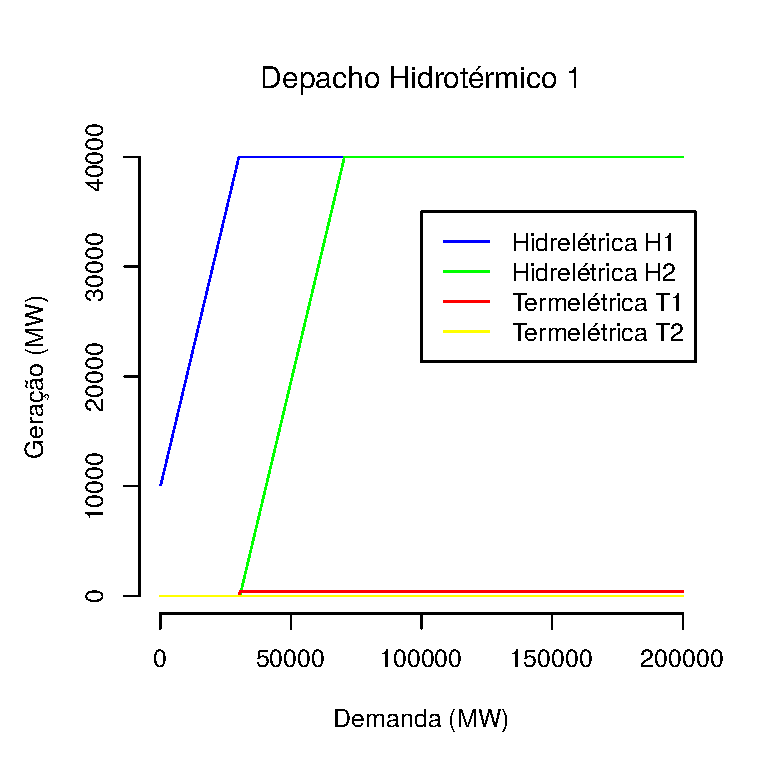
\includegraphics[width=5.0cm, height=4.0cm]{simulacaopb01pt10.eps}}
  \subfigure[Produtibilidade = 1,4.]{
	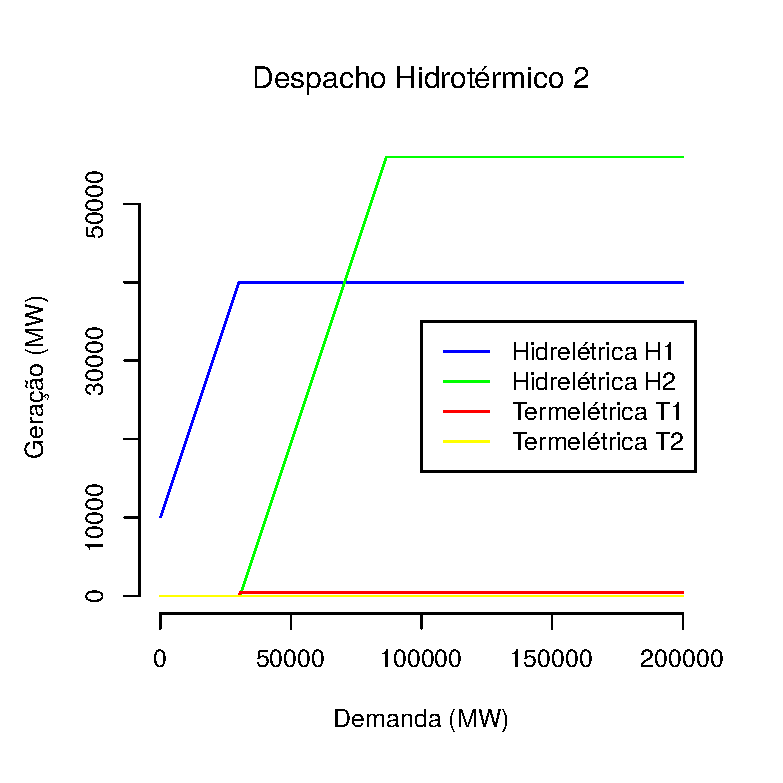
\includegraphics[width=5.0cm, height=4.0cm]{simulacaopb01pt14.eps}}
\subfigure[Produtibilidade = 1,8.]{
	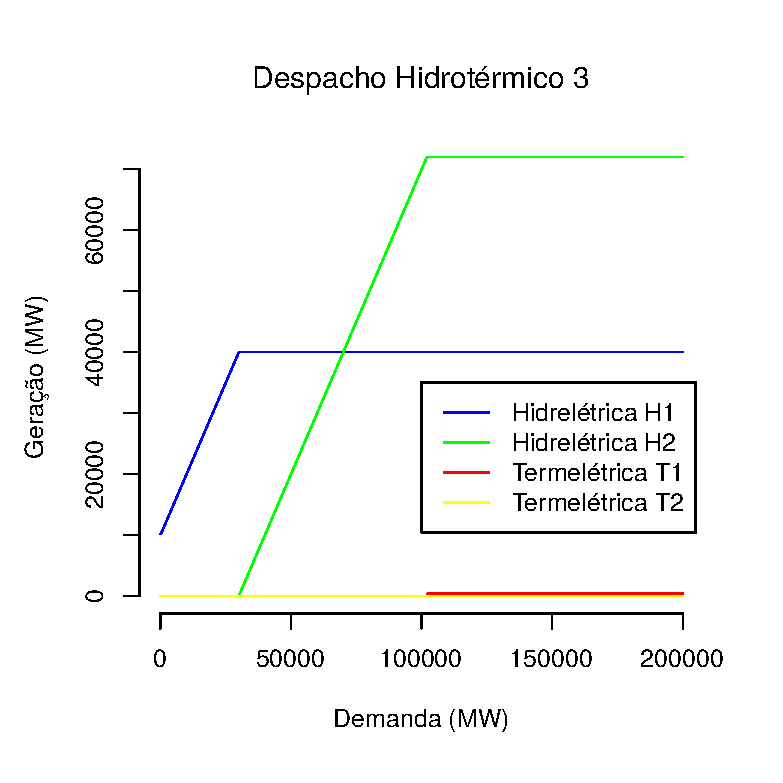
\includegraphics[width=5.0cm, height=4.0cm]{simulacaopb01pt18.eps}}
	\caption{Configura\c c\~ao de despacho para $p = 0,1$ e $1-p = 0,9$.}
	\label{disp1}
\end{figure}

A Figura (\ref{disp1}) \'e constitu\'ida por configura\c c\~oes distintas de planejamento que est\~ao associados a produtibilidade das usinas hidrel\'etricas. Na Figura (\ref{disp1}a) nota-se uma gera\c c\~ao predominantemente da hidrel\'etrica H1 para um intervalo inicial de demanda. Entretanto, a medida que o aumento de demanda torna-se significativo para o sistema ocorre a ativa\c c\~ao da Hidrel\'etrica H2 e da termel\'etrica T1. Observa-se que ocorre um aumento da gera\c c\~ao de H2 e a gera\c c\~ao de T1 permanece constante no per\'iodo de estudo. A Figura (\ref {disp1}b) possui semelhan\c ca ao caso anterior, por\'em  o principal aspecto relevante deve-se a vasta utiliza\c c\~ao da gera\c c\~ao de H2 para essa configura\c c\~ao de despacho. Por fim, a Figura (\ref{disp1}c) possui ampla gera\c c\~ao de H2. Contudo, sua principal caracter\'istica \'e ativa\c c\~ao posterior de T1 em compara\c c\~ao aos outros casos. Em resumo, de acordo com a Figura (\ref{disp1}), a medida que ocorre uma altera\c c\~ao na produtibilidade de H1 e o sistema sofre uma aumento na demanda, o arranjo da gera\c c\~ao \'e alterado.  A an\'alise sobre o impacto que ocorre com o custo em rela\c c\~ao a demanda para configura\c c\~oes de produtibilidade \'e dado a seguir. 
\begin{figure}[!htpb]
\centering
  \subfigure[Produtibilidade = 1,0.]{
	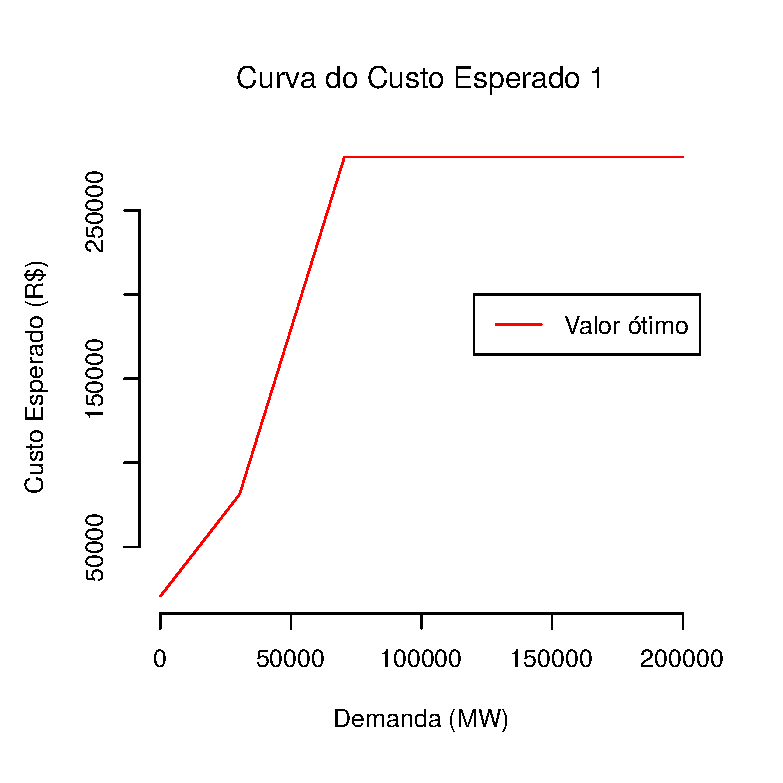
\includegraphics[width=4.0cm, height=4.0cm]{zpb01pt10.eps}}
  \subfigure[Produtibilidade = 1,4.]{
	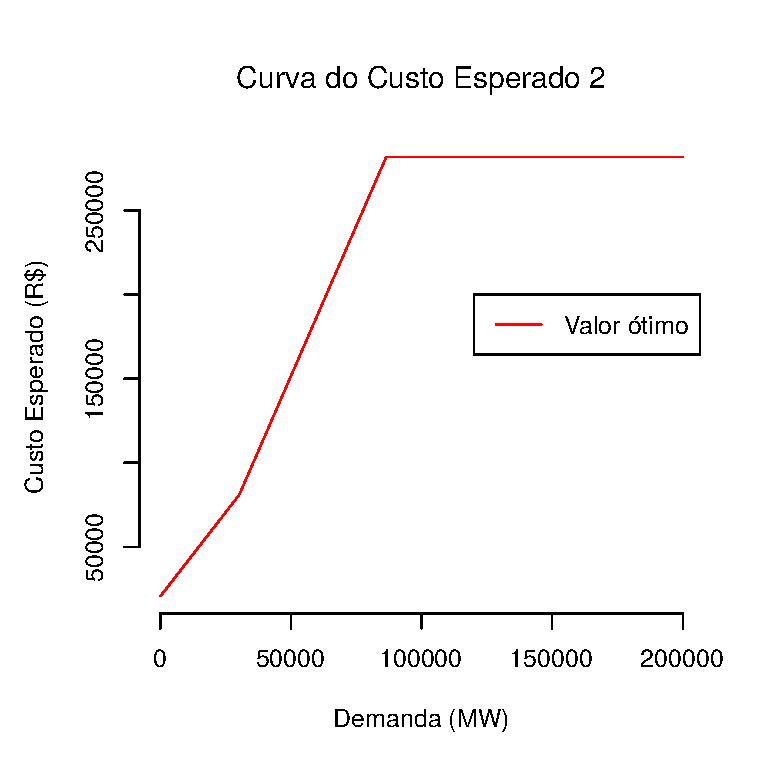
\includegraphics[width=4.0cm, height=4.0cm]{zpb01pt14.eps}}
\subfigure[Produtibilidade = 1,8.]{
	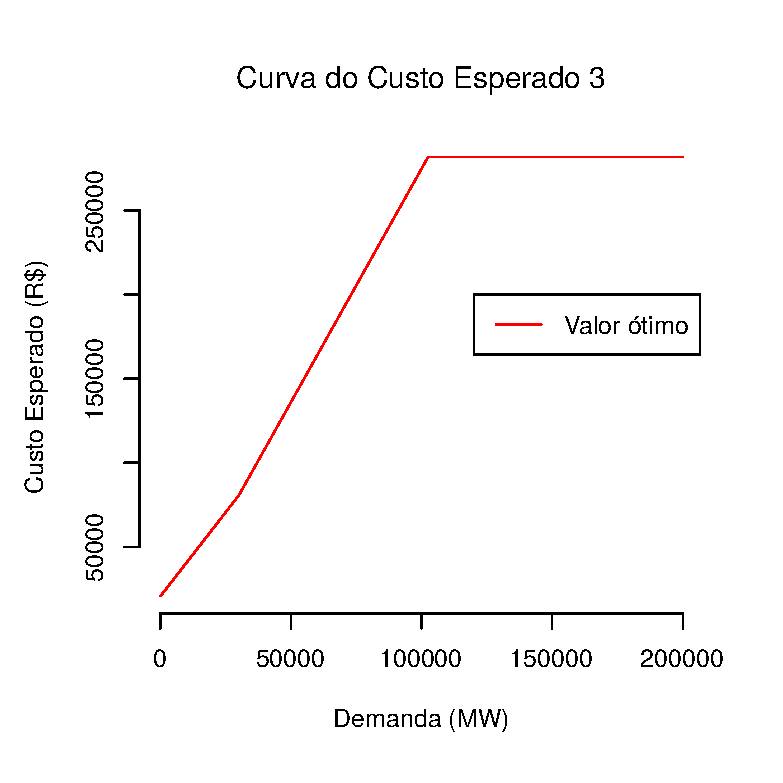
\includegraphics[width=4.0cm, height=4.0cm]{zpb01pt18.eps}}
	\caption{Relação entre demanda e custo esperado $p = 0,1$ e $1-p = 0,9$.}
	\label{cust1}
\end{figure}

Conforme descrito em Figura (\ref{cust1}), as configura\c c\~oes de produtibilidade para aumento da demanda tiveram um
impacto consider\'avel no valor de custo. De fato, percebe-se uma suaviza\c c\~ao da curva do valor \'otimo para o custo
associado ao sistema. No primeiro momento ocorre um crescimento sim\'etrico em ambos os casos descritos na Figura
(\ref{cust1}). Por\'em, a medida que ocorre uma crescimento na demanda. Em determinada ocasi\~ao nota-se uma ruptura na
sim\'etria da curva ocorrendo um aumento do custo. Posteriormente, o equil\'ibrio \'e atingido. A configura\c c\~ao da
produtibilidade considerada de maior import\^ancia para o despacho hidrot\'ermico \'e a encontrada em Figura
(\ref{disp1}c) tamb\'em descrita em Figura (\ref{cust1}c). Pois, nota-se uma adapta\c c\~ao favor\'avel do sistema pelo
aspecto do custo, uma vez que pela suaviza\c c\~ao ocorrida evita-se aumentos inesperados. O segundo ponto  \'e a
relev\^ancia ambiental associada com o uso das termel\'etricas. Visto que, a termel\'etrica T1 \'e ativada em um
per\'iodo posterior em rela\c c\~ao as outras configura\c c\~oes. Desta forma, o sistema utilizando-se da configura\c
c\~ao na Figura (\ref{disp1}) manteve-se em condi\c c\~oes de adapta\c c\~oes para o aumento na demanda. Vale salientar,
que a ruptura observada na Figura (\ref{disp1}) em todos casos deve-se ao \^onus da ativa\c c\~ao de T1. Para a presente
an\'alise considerou-se v\'arios outros cen\'arios com probabilidades distintas. Contudo, pelos resultados no aspecto
geral serem semelhantes esses cen\'arios n\~ao foram descritos no presente trabalho. Por fim, a figura a seguir descreve
de forma b\'asica as configura\c c\~oes encontradas. A configura\c c\~ao satisfat\'oria \'e a segunda.
\begin{figure}[!ht]
    \centering
    \resizebox{0.8\textwidth}{!}{%
\begin{tikzpicture}
  \draw node[draw, circle] (p10) at (1,1) {P = 1.0};
  \draw node[draw, circle] (p14) at (4,1) {P = 1.4};
  \draw node[draw, circle] (p16) at (7,1) {P = 1.6};
  \draw node[draw, circle] (p18) at (10,1) {P = 1.8};
  \draw node[draw, circle] (p20) at (13,1) {P = 2.0};
  \draw [draw] (p10) to [out=0,in=180] (p14);
  \draw [draw] (p14) to [out=0,in=180] (p16);
  \draw [draw] (p16) to [out=0,in=180] (p18);
  \draw [draw] (p18) to [out=0,in=180] (p20);
  \node [draw](S) at (5.5,5.0) {Ativa\c c\~ao simult\^anea};
  \node [draw, circle, minimum size=5.3cm](c1) at (5.5,5.0) {};
  \node [draw, minimum size=1.0cm] (t1) at (4,4) {T1};
  \node [draw, minimum size=1.0cm] (h2) at (7,4) {H2}; 
  \draw [draw] (t1) to [out=0,in=180] (h2); 
  \draw [draw] (p10) to [out=90,in=180] (t1); 
  \draw [draw] (p18) to [out=90,in=0] (h2); 
  \draw node [] at (5.5, 6.5){Configura\c c\~ao 1};
  \draw node[align=center,draw, minimum size=1.5cm](h) at (11.5,6.4) {Prolongada\\ utiliza\c c\~ao \\de H2};  
  \draw [draw] (p18) to [out=90,in=180] (h);
  \draw [draw] (p20) to [out=90,in=0] (h);
  \draw node[align=center,draw, minimum size=1.5cm](t) at (11.5,4.4) {Posterior\\ ativa\c c\~ao \\de T1};  
  \draw [draw] (h) to [out=270,in=90] (t);
  \node [draw, circle, minimum size=5.2cm](c1) at (11.5,5.2) {};
  \draw node [] at (11.5, 3.2){Configura\c c\~ao 2};
  \node [draw,align=justify, minimum size=2cm]() at (1.0,6.0) {P-Produtibilidade\\
  T1-Termel\'etrica 1\\H2-Hidrel\'etrica 2 };
\end{tikzpicture}}

    \caption{Configura\c c\~oes para o despacho hidrot\'ermico.}
\end{figure}
\section{CONCLUS\~OES}
O objetivo deste trabalho foi analisar o comportamento de um sistema hidrot\'ermico sobre as varia\c c\~oes na demanda com rela\c c\~ao as produtibilidades distintas para a descri\c c\~ao do despacho hidrot\'ermico, na  qual a t\'ecnica utilizada foi a Programa\c c\~ao Din\^amica Dual Estoc\'astica. O sistema foi estruturado com duas hidrel\'etricas em cascata H1 e H2 e duas termel\'etricas associadas T1 e T2. Ap\'os a an\'alise dos resultados p\^ode-se verificar que as varia\c c\~oes na demanda podem alterar significativamente o comportamento de sistemas hidrot\'ermicos. Pois, aumentos significativos ocasionaram a ruptura da curva de custo esperado. O principal motivo deve-se ao \^onus do custo associado a gera\c c\~ao da termel\'etrica T1. Entretanto, dada a configura\c c\~ao das produtibilidades das usinas percebeu-se uma mudan\c ca no comportamento do sistema notando-se duas configura\c c\~oes distintas. Para um produtibilidade baixa notou-se a ativa\c c\~ao simult\^anea de T1 e de H2. Por outro lado, com uma produtibilidade elevada o sistema manteve-se com a gera\c c\~ao das hidr\'eletricas H1 e H2 evitando-se a ativa\c c\~ao das term\'eletricas associadas T1 e T2. A segunda configura\c c\~ao considerou-se favor\'avel principalmente pela ativa\c c\~ao tardia de T1 evitando-se preju\'izos ambientais e o aumento no custo esperado. Este trabalho se justifica pela necessidade do planejamento energ\'etico no intuito do uso efi\^enciente da energia e na perspectiva do desenvolvimento sustent\'avel. Por fim, este trabalho est\'a longe de ser um estudo completo sobre o despacho hidrot\'ermio, uma vez que muitas melhorias podem ser feitas. Por exemplo, an\'alise dos volumes iniciais das usinas hidrel\'etricas para diminui\c c\~ao da necessidade de um produtibilidade elevada para uma adpta\c c\~ao favor\'avel do sistema. Al\'em de considerar fontes renov\'aveis como a e\'olica e a solar no
modelamento.
% ------------------------------------------------------------------------
\expandafter\def\expandafter\UrlBreaks\expandafter{\UrlBreaks%  save the current one
  \do\a\do\b\do\c\do\d\do\e\do\f\do\g\do\h\do\i\do\j%
  \do\k\do\l\do\m\do\n\do\o\do\p\do\q\do\r\do\s\do\t%
  \do\u\do\v\do\w\do\x\do\y\do\z\do\A\do\B\do\C\do\D%
  \do\E\do\F\do\G\do\H\do\I\do\J\do\K\do\L\do\M\do\N%
  \do\O\do\P\do\Q\do\R\do\S\do\T\do\U\do\V\do\W\do\X%
  \do\Y\do\Z}
\section*{REFER\^ENCIAS}

\begin{description}[noitemsep, labelindent=-0.2cm,leftmargin=0.4cm]
\fontsize{11}{0}\selectfont
\item
Ag\^encia Nacional de Energia El\'etrica (2008), Atlas de Energia Elétrica do Brasil, 3.ed., Brasília.
\item
Benders, J. F. (1962), Partitioning procedures for solving mixed-variables programming problem. Numerische Mathematik,
vol 4, 238-252.
\item
Centro de Pesquisas de Energia Elétrica (2001), Modelo DECOMP CEPEL: Manual de refer\^encia.
\item
Cerisola, S.; Latorre, J.M; Ramos, A. (2012), Stochastic dual dynamic programming applied to nonconvex hydrothermal models.
European Journal of Operational Research, vol 218, 687-697.
\item
Izmailov, A.; Solov, M. (2014), {\em Otimiza\c c\~ao volume 1. Condi\c c\~oes de otimalidade, Elementos de An\'alise Convexa e
de Dualidade}. 3 ed, Rio de Janeiro: IMPA. 
\item
Martinez, L.; Soares, S. (2004), ``Primal and dual stochastic dynamic programming in long term hydrothermal scheduling''.
{\em IEEE PES Power Systems Conference and Exposition}.
\item
Rebennack, S. (2016), Combining  sampling-based and scenario-based nested Benders decomposition methods: application to
stochastic dual dynamic programming. Mathematical Programming, vol 156, 343-389. 
\item
Santos, J.B. Despacho Hidrot\'ermico de Energia. Dispon\'ivel em : https://github.com/Jeffreypir/Modela-gem. Acesso em: 20 de Ago. de 2019.
\item
  Tolmasquim, M. (2016), {\em Energia Termel\'etrica: G\'as Natural, Biomassa, Carv\~ao, Nuclear}. EPE: Rio de Janeiro.
\end{description}
\vspace*{-0.1cm}
% ------------------------------------------------------------------------

%For papers written in Portuguese or Spanish.

\begin{center}
 \textbf {A COMPUTATIONAL CASE OF STUDY FOR ELECTRIC DISPATCH IN A HYDROTHERMAL MODEL}
\end{center}

\def\abstractname{Abstract}%

\begin{abstract}
In the last decades, the demands for renovable sources of electrical energy have increased. Hence, big technological advances have been essential, in order to have an efficient and sustainable electrical system. In Brazil , the hydroelectric source is the most important one. However, the unproportional demands and the low level of water reservoir have implied to use thermolelectric source. Therefore, who pay the bill are the costumers. With this in mind, this work has as goals: to analazy the consequences with the demands increaseing and changes of producibility, in the scenary of energetic problems and which can be induced in the energetic balance. The most important point must be to forsee how to manage the energetic system which we call the eletric dispatch. Always trying to minimize the costs and the decreasing of the enviromental impact. This text can be seen as a case of study about hydrothermal systems using Stochastic Dual Dynamical Programming. In fact, both demand and producibility are changed, then we obtain the best combination that implies the dispatch choice with the minimum cost expectation for the system. 

\end{abstract}

\keywords{\em{Power generation, Demand, Hydrothermal Model, 
Planning, Dual Dynamic Stochastic Programming.}}

\end{document}
